\usepackage{graphicx}\thispagestyle{fancy}

\vspace{\fill}


\section{\makeUppercase{\large{Descrição das telas}}}

%Here is where the screen's description  has to be inputed
Para permitir remover todos os botões de comando da máquina, foi levado muito a sério a facilidade de navegação entre as telas.
No canto superior direito encontramos um pequeno menu contendo o botão de salvar que quando pressionado grava o ajuste atual da
máquina na receita carregada. A sua esquerda se encontra o botão de acesso a tela de velocidade.
O botão de alarmes no canto inferior direito leva a sua respectiva tela e quando está piscando na cor alaranjada significa
que tem um alarme ativo. Exceto o botão ajuda, descreverei os próximos futuramente, ao clicar em ajuda será descrito as
funções da tela ativa, como mostrado nas próximas imagens.

\subsection{Ajuda tela Principal}
A tela principal contém informações do pedido atual e dos ultimos pedidos rodados. Também
possui informações de quais impressoras estão habilitadas e que cor está configurada.

\begin{figure}
    \centering
    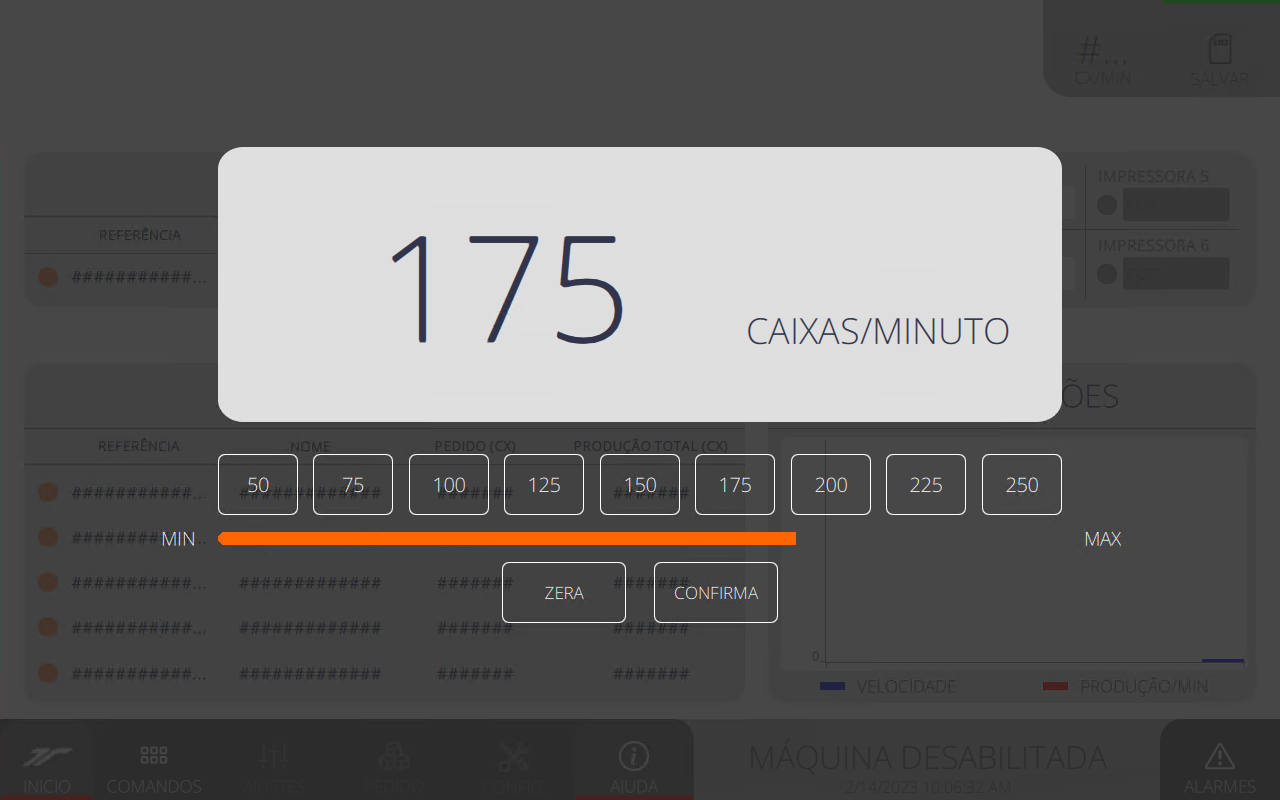
\includegraphics[width=576,height=360,angle=0]{imagesICV/01-main/1}
    \caption{Tela principal}
    \label{fig:}
\end{figure}

\newpage
\thispagestyle{fancy}
\vspace{\fill}

\subsection{\small{Gráficos de velocidade e produção}}

\begin{figure}
    \centering
    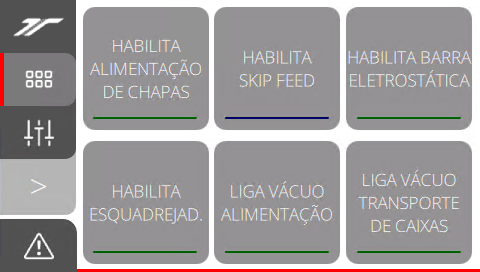
\includegraphics[width=576,height=360]{imagesICV/01-main/2}
    \caption{Informações da máquina}
    \label{fig:}
\end{figure}

\newpage
\thispagestyle{fancy}
\vspace{\fill}

\subsection{\small{Informações das impressoras}}

\begin{figure}
    \centering
    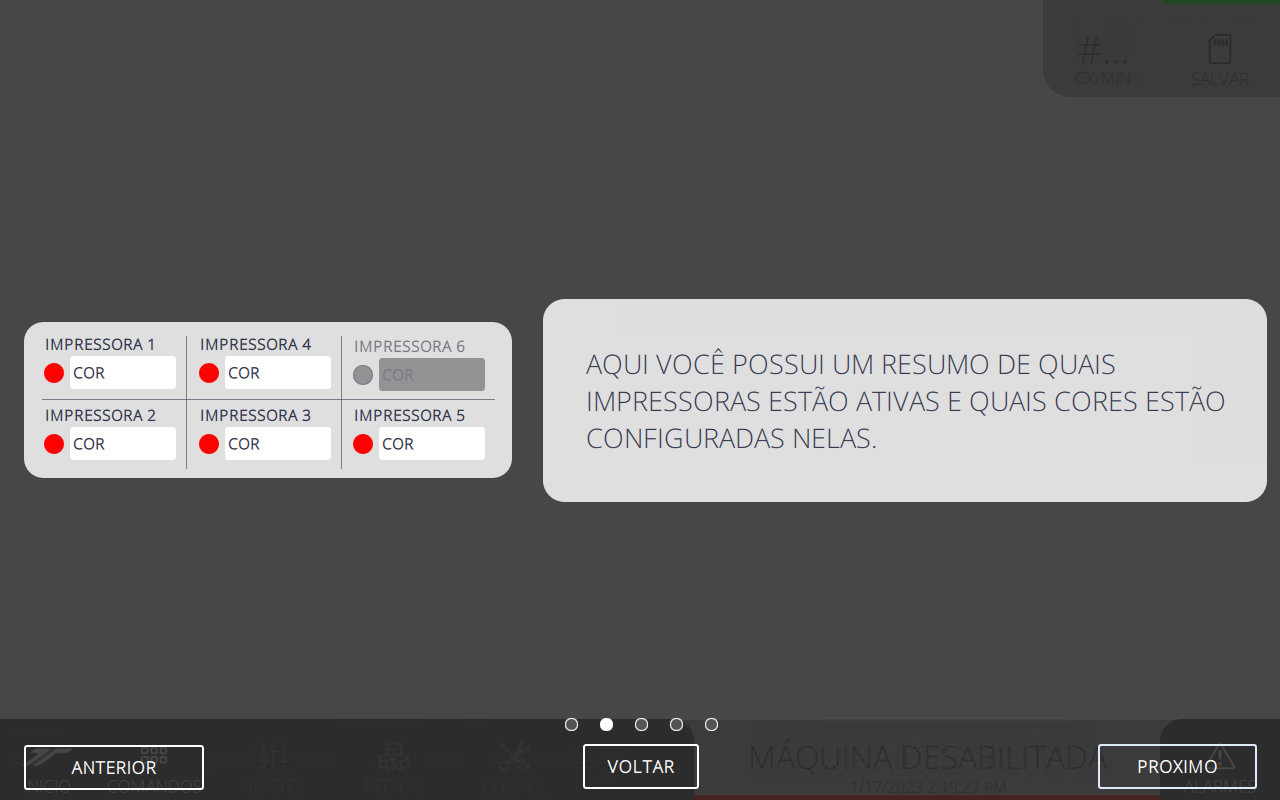
\includegraphics[width=576,height=360]{imagesICV/01-main/3}
    \caption{Informações das impressoras}
    \label{fig:}
\end{figure}

\newpage
\thispagestyle{fancy}
\vspace{\fill}

\subsection{\small{Últimos pedidos}}

\begin{figure}
    \centering
    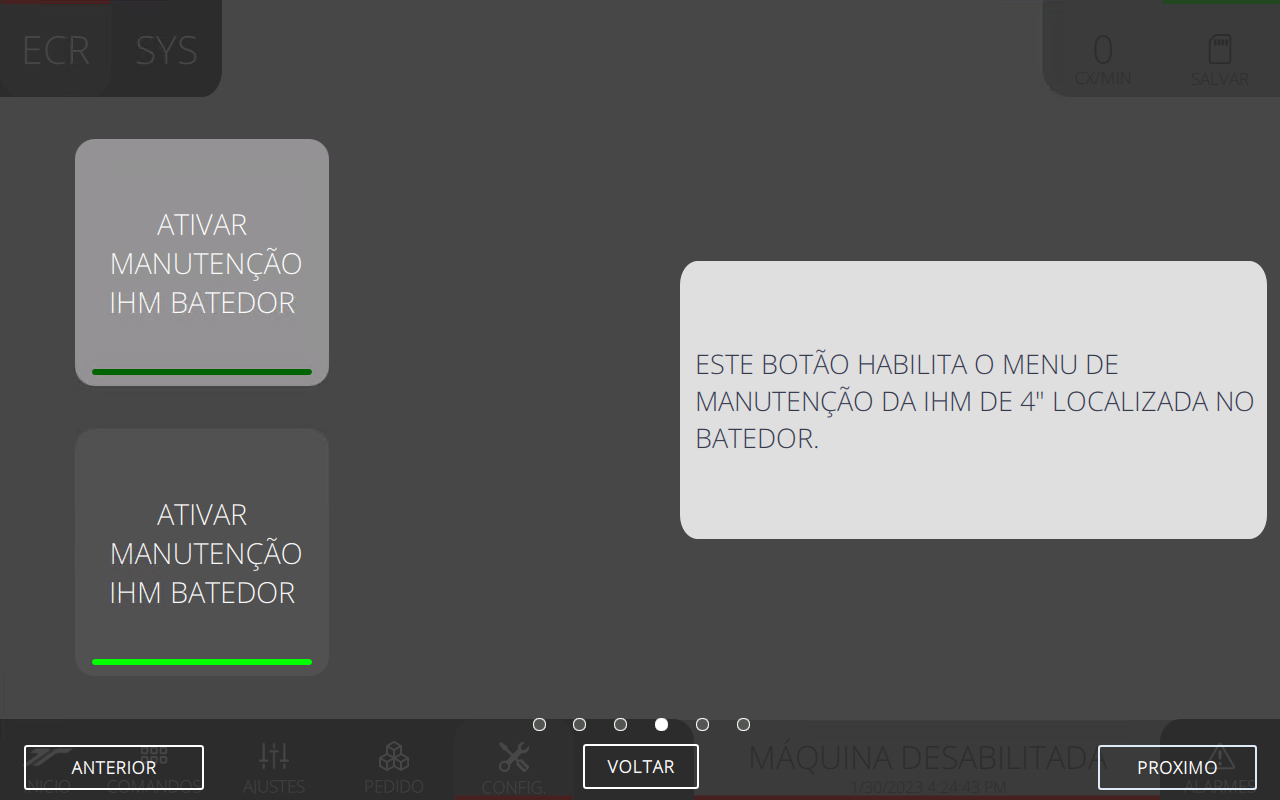
\includegraphics[width=576,height=360]{imagesICV/01-main/4}
    \caption{Vista da tela pré rodagem dos pedidos}
    \label{fig:}
\end{figure}

\newpage
\thispagestyle{fancy}
\vspace{\fill}

\subsection{\small{Últimos pedidos}}

\begin{figure}
    \centering
    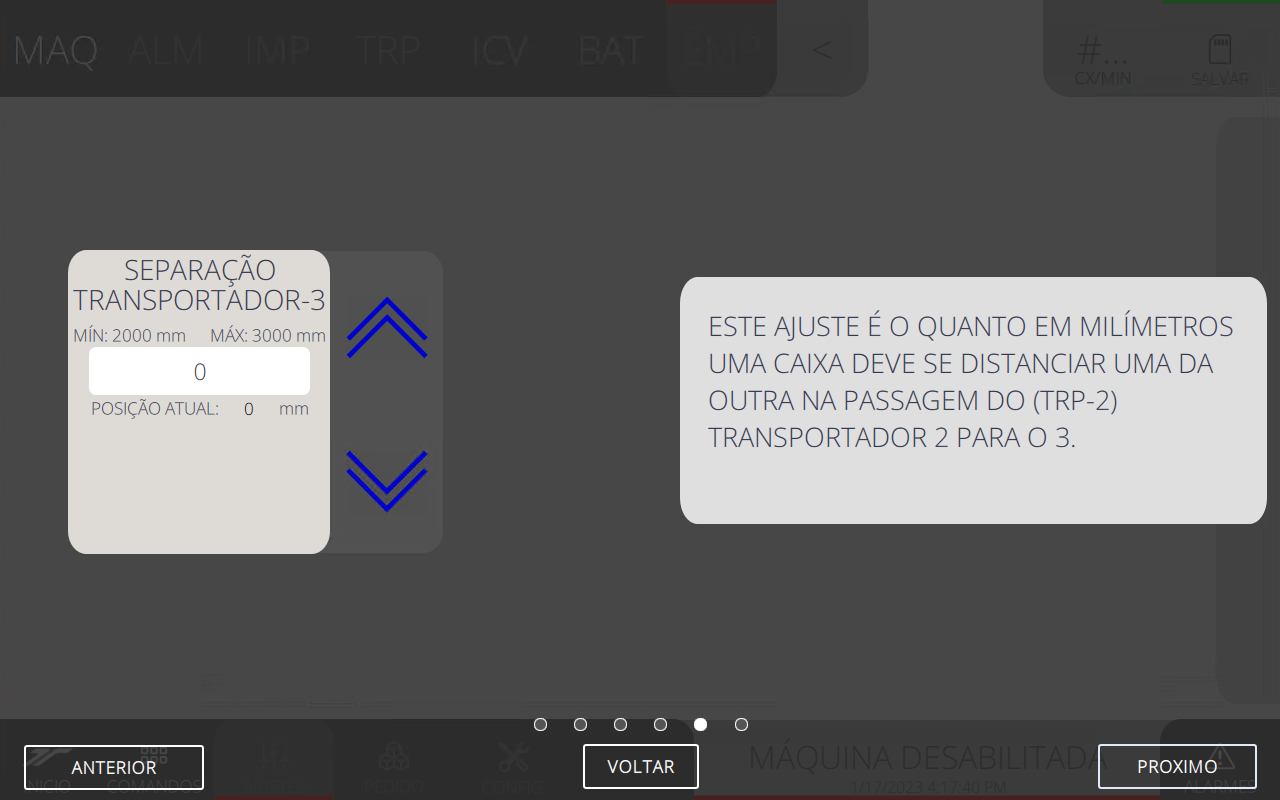
\includegraphics[width=576,height=360]{imagesICV/01-main/5}
    \caption{Vista da tela pós rodagem dos pedidos}
    \label{fig:}
\end{figure}

\newpage
\thispagestyle{fancy}
\vspace{\fill}

\subsection{\small{Produção atual}}

\begin{figure}
    \centering
    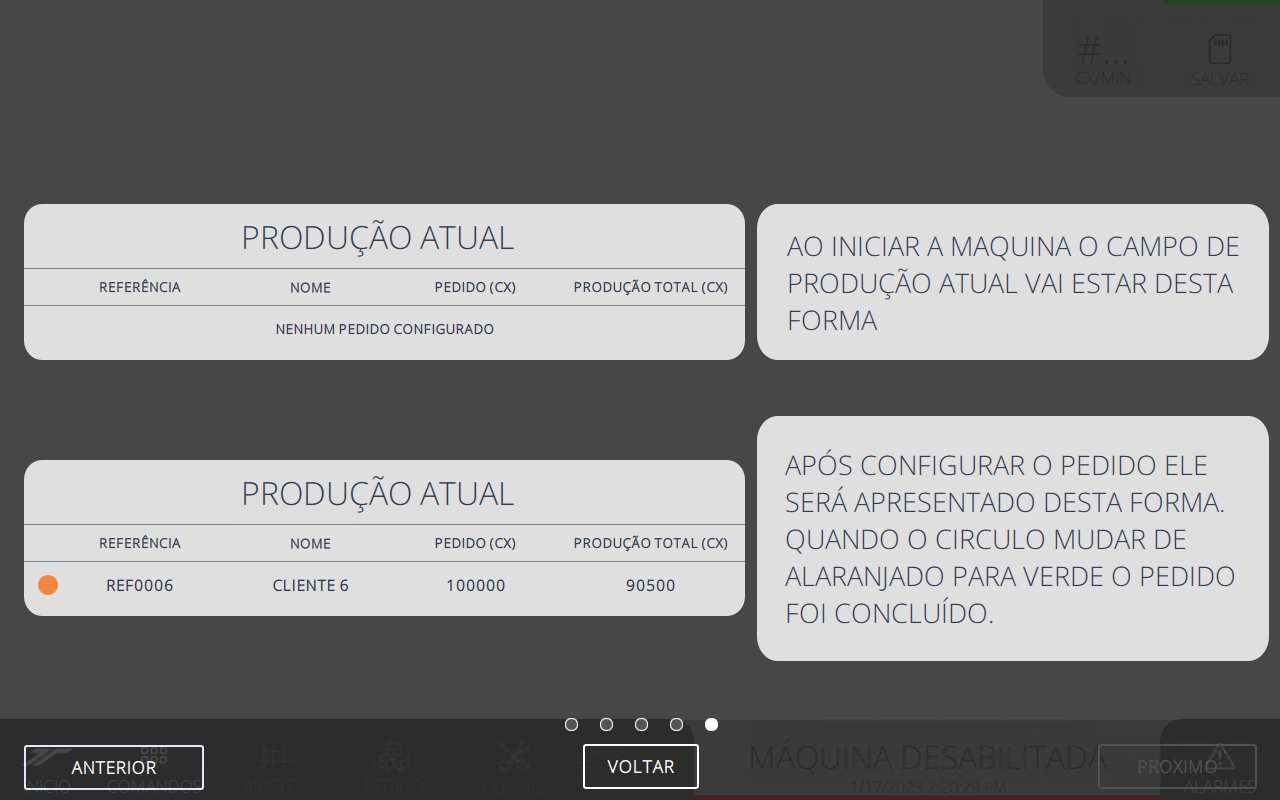
\includegraphics[width=576,height=360]{imagesICV/01-main/6}
    \caption{Status da produção}
    \label{fig:}
\end{figure}
